\documentclass[titlepage,a4paper]{article}

\usepackage{a4wide}
\usepackage[colorlinks=true,linkcolor=black,urlcolor=blue,bookmarksopen=true]{hyperref}
\usepackage{bookmark}
\usepackage{fancyhdr}
\usepackage[spanish]{babel}
\usepackage[utf8]{inputenc}
\usepackage[T1]{fontenc}
\usepackage{graphicx}
\usepackage{float}

\pagestyle{fancy} % Encabezado y pie de página
\fancyhf{}
\fancyhead[L]{TP2 - Grupo 05}  % CAMBIAR NOMBRE
\fancyhead[R]{Paradigmas De la Programacion - FIUBA}
\renewcommand{\headrulewidth}{0.4pt}
\fancyfoot[C]{\thepage}
\renewcommand{\footrulewidth}{0.4pt}
\usepackage{listings}
\usepackage{xcolor}

\begin{document}
	\begin{titlepage} % Carátula
		\hfill
\includegraphics[width=6cm]{logofiuba.jpg}
		\centering
		\vfill
		\Huge \textbf{Trabajo Práctico 2 — Gwent}
		\vskip2cm
		\Large [7507/9502] {Paradigmas De la Programacion}\\
		Primer cuatrimestre de 2025 % Ajustar cuatrimestre
		\vfill
		\begin{tabular}{ | l | l | l | } % Nueva tabla con encabezados
			\hline
			\textbf{Alumno} & \textbf{Número de padrón} & \textbf{Email} \\ \hline
			Sebastian Colazo & 111737 & scolazo@fi.uba.ar \\ \hline
			Nahuel Giner & 111884 & nginer@fi.uba.ar\\ \hline
			Aksel Mendoza & 108171 & aemendoza@fi.uba.ar \\ \hline
			Miguel Zorrilla & 110619 & mzorrilla@fi.uba.ar  \\ \hline
			Iñaki Vydra & 111505 & ivydra@fi.uba.ar \\ \hline
		\end{tabular}
		\vfill
	\end{titlepage}
	
	\tableofcontents % Índice general
	\newpage
	
	\section{Introducción}\label{sec:intro}
	El presente informe reune la documentación de la solución del segundo trabajo práctico de la materia Paradigmas De la Programacion que consiste en desarrollar una aplicacion completa del juego de cartas \textbf{Gwent}, aplicando todos los conceptos vistos en
	el curso, utilizando el lenguaje Java con un diseño del modelo orientado a objetos y trabajando con las tecnicas de TDD e Integración Continua.


	\section{Detalles de implementación}\label{sec:implementacion}

	\subsection{Supuestos}\label{sup:intro}
	\begin{itemize}
		\item \textbf{Médico:} El modificador \textit{Médico} permite agarrar una carta de la pila de descarte y jugarla en el momento.
		En nuestra implementación, se asume que la carta que se recupera es siempre la última unidad descartada. Esta elección simplifica la interacción y mantiene la dinámica del juego fluida. En la interfaz gráfica, se muestra la pila de descarte de cada jugador, lo que permite visualizar claramente cuál será la carta que será revivida.

		\item \textbf{Nombres:} Las cartas, tanto especiales como de unidad, tienen un nombre asociado. Para poder crear las vistas de las cartas, asumimos que todas las cartas con el mismo nombre deben representarse de la misma manera, es decir, con la misma descripción e imagen. Esta suposición nos permitió asociar un estilo visual único a cada nombre, simplificando la construcción de vistas carta.

	\end{itemize}

	\subsection{Delegación vs Herencia}\label{sup:vs}
	En general, evitamos el uso de herencia ya que implica una relacion fuerte y rigida entre las clases pero la utilizamos para modelar la jerarquia entre \texttt{Carta} y \texttt{Unidad}, ya que una unidad es un tipo de carta. Lo mismo aplica para las \texttt{UnidadesModificadas}, ya que necesitabamos una clase base comun desde la cual poder aplicar los distintos modificadores.
	Para el resto del diseño optamos por la delegación, ya que nos da mayor flexibilidad y favorece la composición de comportamientos sin acoplar fuertemente las clases.

	\subsection{Puntos conflictivos}\label{sup:conflicto}

	Uno de los aspectos más complejos del trabajo práctico fue la programación de las secciones del tablero de cada jugador y la lógica de las unidades, ya que el puntaje de una sección depende de las unidades que contiene, pero a su vez, el puntaje de cada unidad puede depender del estado actual de la sección en la que está colocada.
	Por ejemplo, el puntaje de una unidad puede verse modificado si en la misma sección hay una unidad animadora, o si la sección está afectada por cartas especiales como \textit{climas} o \textit{morale boost}.
	Para resolver este problema, decidimos que sea la sección calcule su puntaje como la suma de los puntajes de sus unidades colocadas y dejar que cada unidad calcule su puntaje pasandole las unidades y efectos en la seccion en ese momento.
	De esta forma, la sección no necesita conocer los tipos específicos de unidades ni los efectos que la afectan; simplemente almacena sus componentes y delega el cálculo a quienes los conocen, lo cual es fundamental para que el diseño sea extensible.


	\subsection{Patrones de diseño}\label{sup:patrones}

	\begin{itemize}
		\item \textbf{Observer:} \\
		Se utilizó el patrón \textit{Observer} para actualizar las vistas correspondientes a la mano, las secciones del tablero y los mazos de los jugadores. Este patrón nos permitió suscribir las vistas a las clases del modelo, de modo que puedan ser notificadas automáticamente ante cambios relevantes, como por ejemplo cuando un jugador roba cartas de su mazo o cuando se agrega una unidad a una sección del tablero.

		\item \textbf{Singleton:} \\
		El patrón \textit{Singleton} fue aplicado para implementar una especie de \textit{cache} de constructores de vistas de cartas. Durante el proceso de parseo del GWENT.JSON con los datos de las cartas, se crea una instancia del modelo correspondiente a cada carta. Sin embargo, ciertos atributos como la descripción y el tipo de una carta especial o la imagen de las cartas son datos que se deben mostrar en la vista, pero que no deberían formar parte del modelo, ya que lo contaminarían con información propia de la interfaz.
		Para resolver este problema, definimos estilos de vista para cada carta, que encapsulan esta información visual y saben construir una vista de carta a partir de una instancia del modelo. Utilizamos el nombre de la carta como identificador (ID), y al leer el JSON cargamos en \texttt{CacheEstilosVistaCarta} las configuraciones necesarias para representar visualmente cada carta según su nombre (ID).
		Era necesario que esta cache tuviera una única instancia accesible desde cualquier vista que necesitara mostrar cartas, por lo que la utilización del patrón \textit{Singleton} resultó una solución adecuada.

		\item \textbf{Template + Decorator:} \\
		Crear las unidades y sus modificadores fue uno de los desafíos más complejos del trabajo, ya que constituyen uno de los aspectos centrales del juego. Un buen modelo debía permitir extender fácilmente la cantidad de modificadores que se pueden aplicar a las cartas.
		Inicialmente probamos enfoques como el patrón \textit{Strategy}, permitiendo que cada modificador implemente su propia lógica sobre cómo debe jugarse la carta. Sin embargo, optamos por utilizar el patrón \textit{Decorator}, ya que nos permitía tomar una unidad base y agregarle funcionalidades adicionales a sus métodos, lo cual encajaba perfectamente con la idea de los modificadores. Como ventaja adicional, nos permitió combinar múltiples modificadores de forma muy sencilla, simplemente decorando una unidad ya decorada.
		Complementamos esta solución con el patrón \textit{Template Method}, que define una estructura base para el comportamiento general de una unidad al ser jugada. Cada modificador puede intervenir decorando sólo las partes relevantes de esa estructura, permitiendo un código limpio y modular, donde cada clase de modificador declara únicamente lo que difiere del comportamiento base.


		\begin{lstlisting}[language=Java, caption={Ejemplo de patrón Template + Decorator en una carta con modificador Espia}]
// En la interfaz Unidad
@Override
default void jugarCarta(Jugador jugador, Jugador oponente, Posicion posicionElegida) {
    if (!sePuedeColocar(posicionElegida)) {
        throw new UnidadNoPuedeSerJugadaEnEsaPosicion("");
    }
    Atril atrilDestino = atrilDestino(jugador, oponente);
    atrilDestino.colocarUnidad(this, posicionElegida);
    realizarAccionAdicional(jugador, oponente, atrilDestino, posicionElegida);
}

// En el decorador Espia
@Override
public Atril atrilDestino(Jugador jugador, Jugador oponente) {
    return oponente.getAtril(); // Coloca la unidad en el campo del oponente
}

@Override
public void realizarAccionAdicional(Jugador jugador, Jugador oponente,
                                    Atril atril, Posicion posicionElegida) {
    jugador.robarCartasDelMazo(CANTIDAD_DE_CARTAS_PARA_ROBAR);
    super.unidad.realizarAccionAdicional(jugador, oponente, atril, posicionElegida);
}
		\end{lstlisting}
El ultimo llamado a super.unidad.realizarAccionAdicional(...) se utiliza para continuar la cadena en el caso de que la carta tenga mas modificadores.

		\item \textbf{Factory Method:} \\
		El patrón \textit{Factory Method} fue utilizado para proporcionar una interfaz clara y flexible a la hora de crear unidades del juego. Debido a la posibilidad de combinar múltiples modificadores, la construcción manual de una unidad podía volverse confusa o tediosa.

		Por ejemplo, si deseamos crear una unidad de fuerza 5, ubicada en la posición Cuerpo a Cuerpo, con los modificadores de Ágil (en posición Asedio), Espía y Legendaria, sin una fábrica tendríamos que escribir algo como lo siguiente:

		\begin{lstlisting}[language=Java, caption={Ejemplo de creación de unidad sin usar UnidadFactory}]
Unidad nuevaUnidad = new UnidadBasica("nombre", 5, new CuerpoACuerpo());
Unidad unidadAgil = new Agil(nuevaUnidad, new Asedio());
Unidad unidadAgilYEspia = new Espia(unidadAgil);
Unidad unidadAgilEspiaYLegendaria = new Legendaria(unidadAgilYEspia);
		\end{lstlisting}

		Para simplificar este proceso, implementamos una clase \texttt{UnidadFactory} que permite construir unidades utilizando listas de modificadores y posiciones. De esta forma, el mismo ejemplo se puede expresar de manera mucho más legible:

		\begin{lstlisting}[language=Java, caption={Ejemplo de creación de unidad usando UnidadFactory}]
 modificadores = new ArrayList<>(List.of("Agil", "Espia", "Legendaria"));
 posiciones = new ArrayList<>(List.of("cuerpo a cuerpo", "asedio"));
 Unidad unidad = UnidadFactory.crear("nombre", 5, modificadores, posiciones);
		\end{lstlisting}

	\item \end{itemize}


	\section{Diagramas}\label{sec:diagramas}


	\subsection{Diagramas de clase}\label{sec:diagramasdeclase}

	\begin{figure}[H]
		\centering
		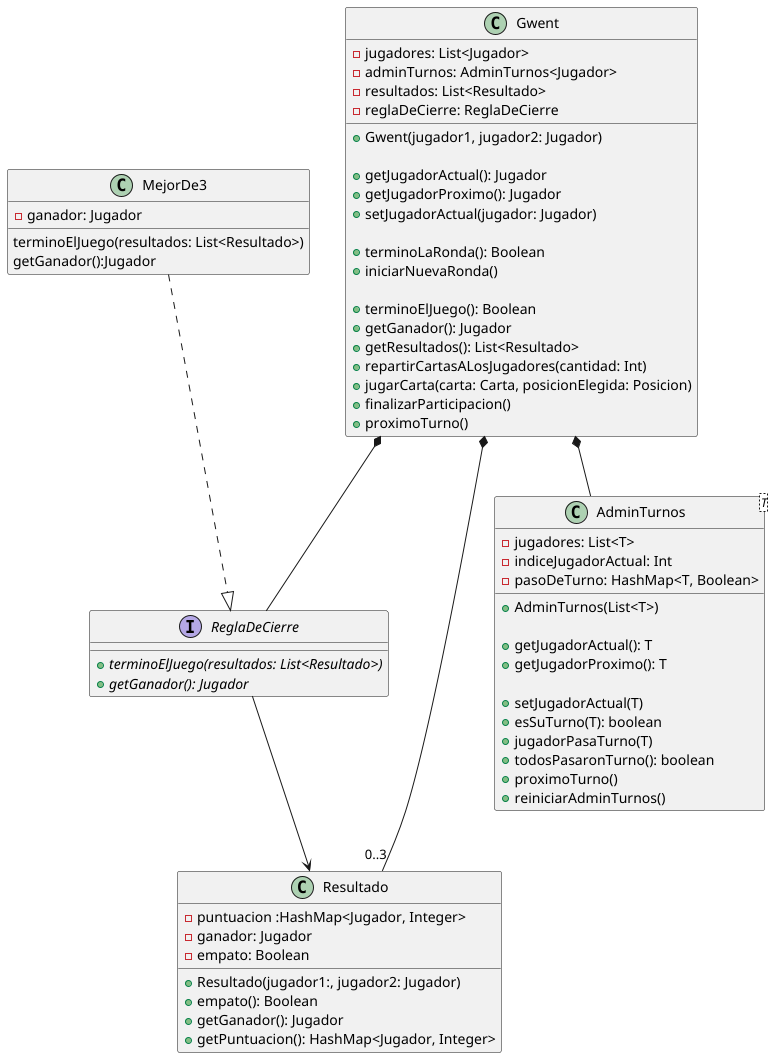
\includegraphics[width=0.8\textwidth]{diagramas/clases/Gwent}
		\caption{\label{fig:class01}Juego \texttt{Gwent}.}
	\end{figure}

	En este diagrama se muestran las clases utilizadas para administrar los turnos y las rondas del juego.
	El \texttt{AdministradorDeTurnos} permite detectar si los jugadores han pasado su turno, y cuando ambos lo hacen, se genera un objeto de tipo \texttt{Resultado}, que contiene el estado actual de los jugadores, sus puntajes en ese momento y quién ganó la ronda.
	Luego, esa información se pasa a una \texttt{ReglaDeCierre}, que se encarga de determinar si el juego debe finalizar o continuar con una nueva ronda.

	\begin{figure}[H]
		\centering
		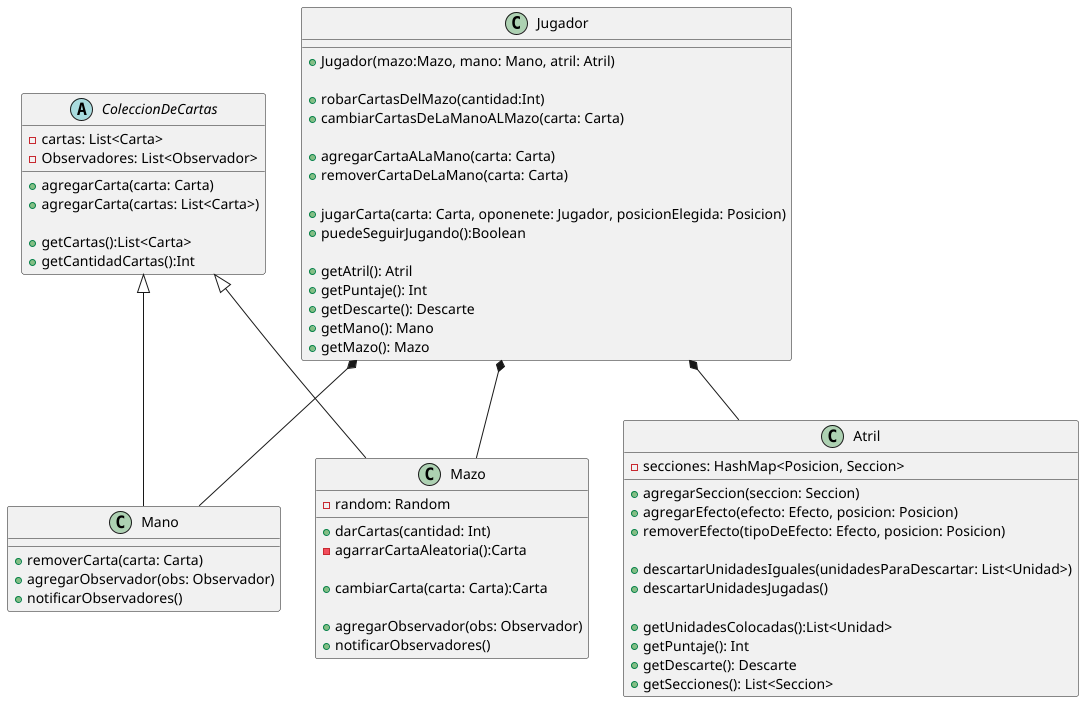
\includegraphics[width=1\textwidth]{diagramas/clases/Jugador}
		\caption{\label{fig:class02}Jugador \texttt{Gwent}.}
	\end{figure}

	\begin{figure}[H]
		\centering
		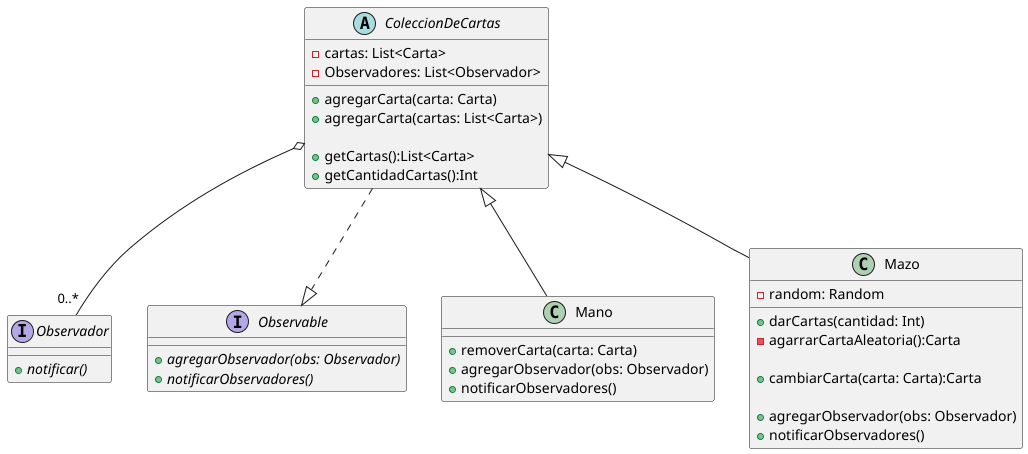
\includegraphics[width=0.8\textwidth]{diagramas/clases/ColeccionDeCartas}
		\caption{\label{fig:class03} ColeccionDeCartas \texttt{Gwent}.}
	\end{figure}

	\begin{figure}[H]
		\centering
		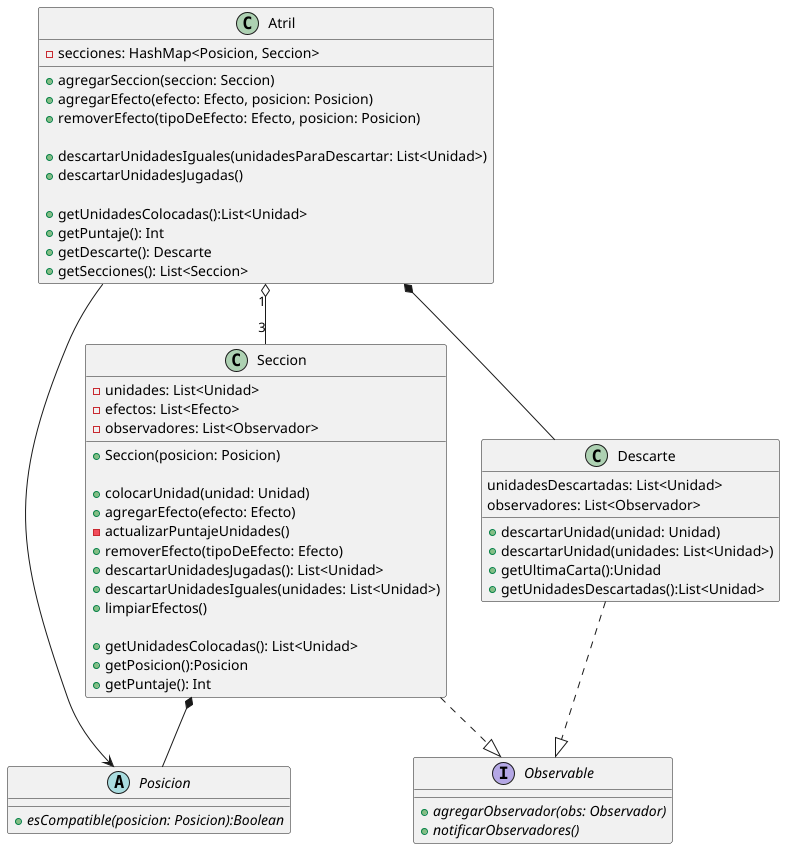
\includegraphics[width=0.8\textwidth]{diagramas/clases/Atril}
		\caption{\label{fig:class04}  \texttt{atril}.}
	\end{figure}


	\begin{figure}[H]
		\centering
		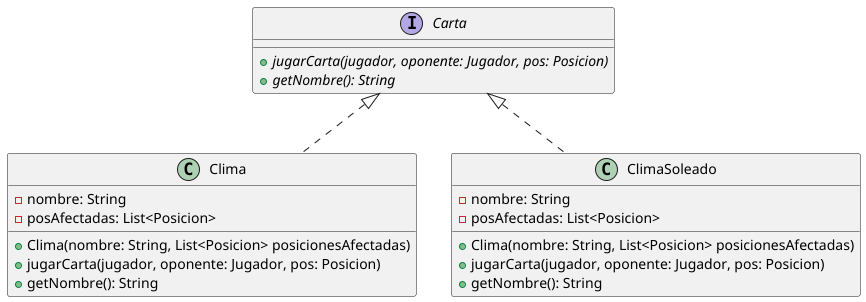
\includegraphics[width=0.8\textwidth]{diagramas/clases/Especiales1}
		\caption{\label{fig:class05} Cartas \texttt{Especiales}.}
	\end{figure}

	\begin{figure}[H]
		\centering
		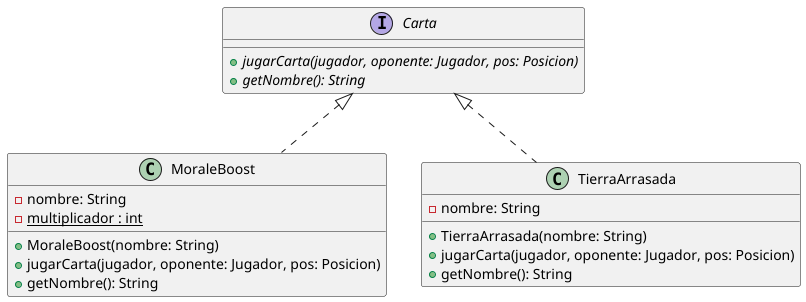
\includegraphics[width=0.8\textwidth]{diagramas/clases/Especiales2}
		\caption{\label{fig:class052} Cartas \texttt{Especiales}.}
	\end{figure}

	\begin{figure}[H]
		\centering
		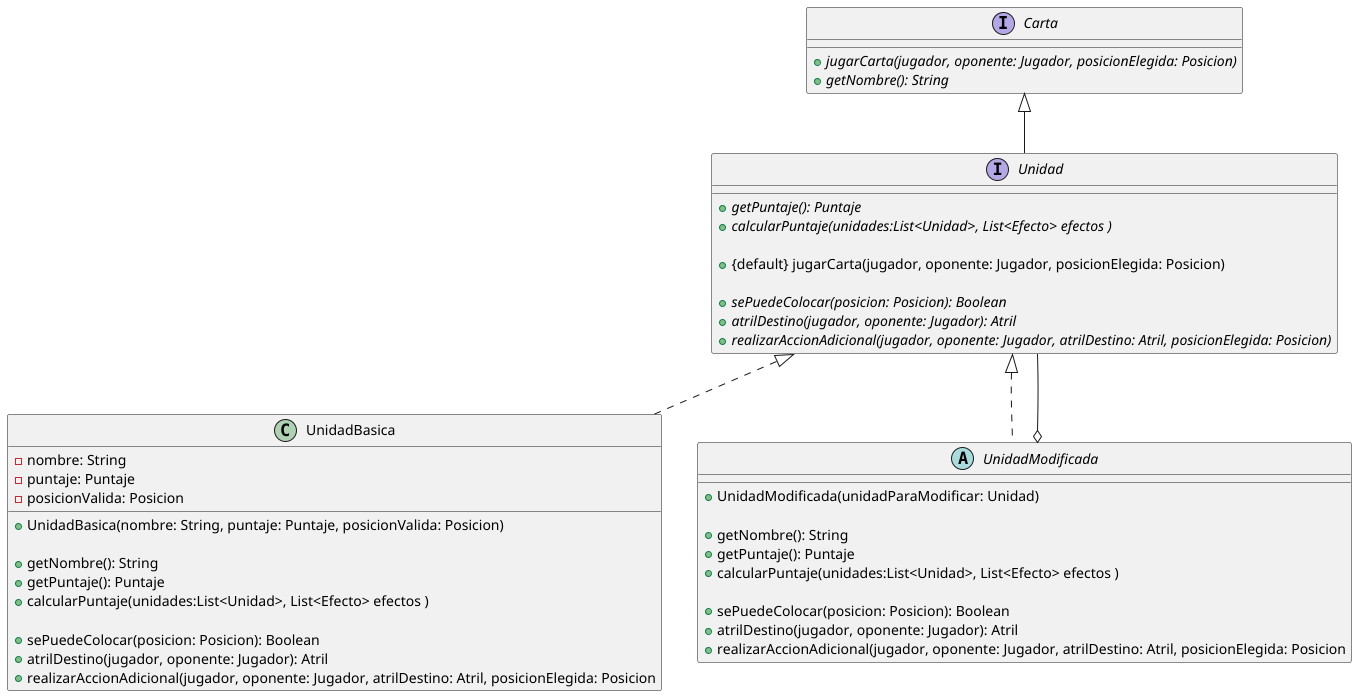
\includegraphics[width=1\textwidth]{diagramas/clases/UnidadBasica}
		\caption{\label{fig:class06}Cartas unidad \texttt{UnidadBasica}.}
	\end{figure}

	La clase \texttt{UnidadBasica} representa una unidad sin modificadores, y funciona como la base sobre la cual pueden aplicarse distintos modificadores.
	Por otro lado, la clase \texttt{UnidadModificada} implementa las interfaces \texttt{Unidad} y \texttt{Carta}, y contiene una referencia a otra unidad.
	Esto le permite delegar sus mensajes a la unidad que envuelve y modificar su comportamiento, agregando lógica adicional antes o después de invocar los métodos originales.

	\begin{figure}[H]
		\centering
		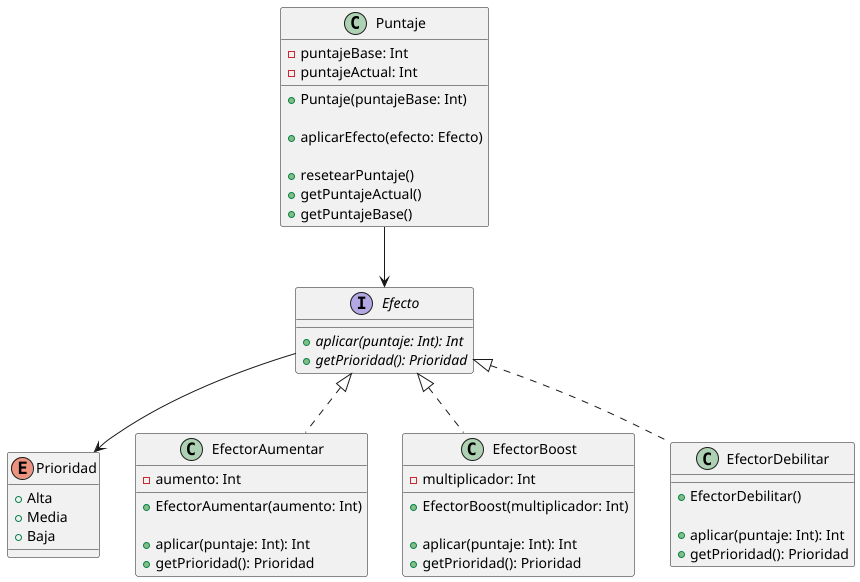
\includegraphics[width=1\textwidth]{diagramas/clases/Puntaje}
		\caption{\label{fig:class07}\texttt{Puntaje}.}
	\end{figure}

	\begin{figure}[H]
		\centering
		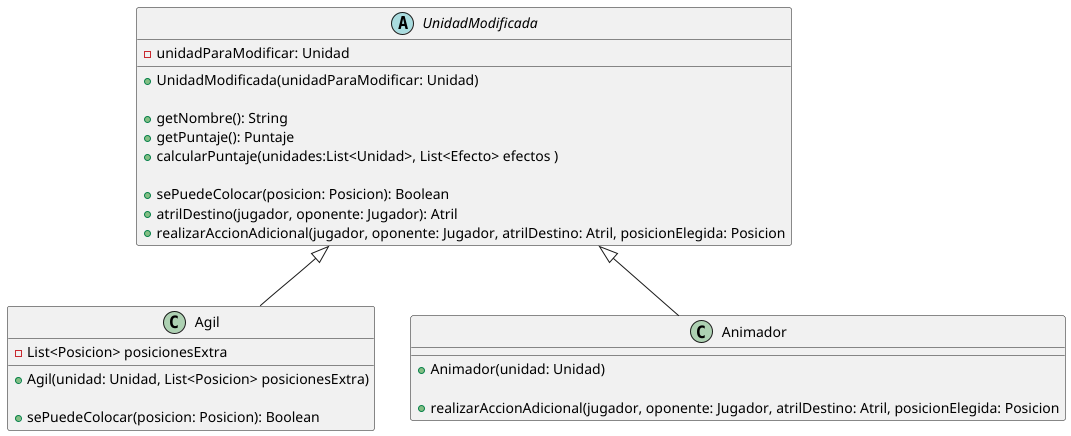
\includegraphics[width=1\textwidth]{diagramas/clases/Modificadores1}
		\caption{\label{fig:class081}Cartas unidad \texttt{Modificadores}.}
	\end{figure}

	\begin{figure}[H]
		\centering
		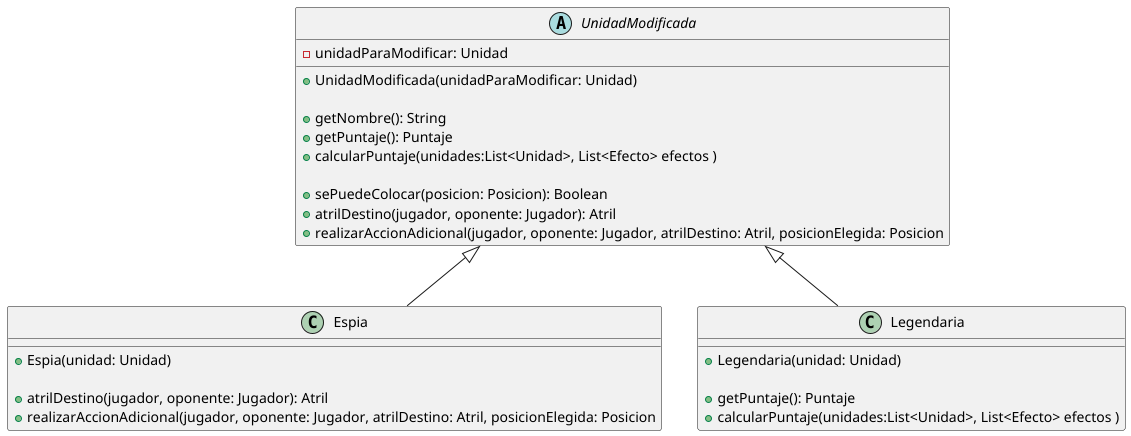
\includegraphics[width=1\textwidth]{diagramas/clases/Modificadores2}
		\caption{\label{fig:class082}Cartas unidad \texttt{Modificadores}.}
	\end{figure}

	\begin{figure}[H]
		\centering
		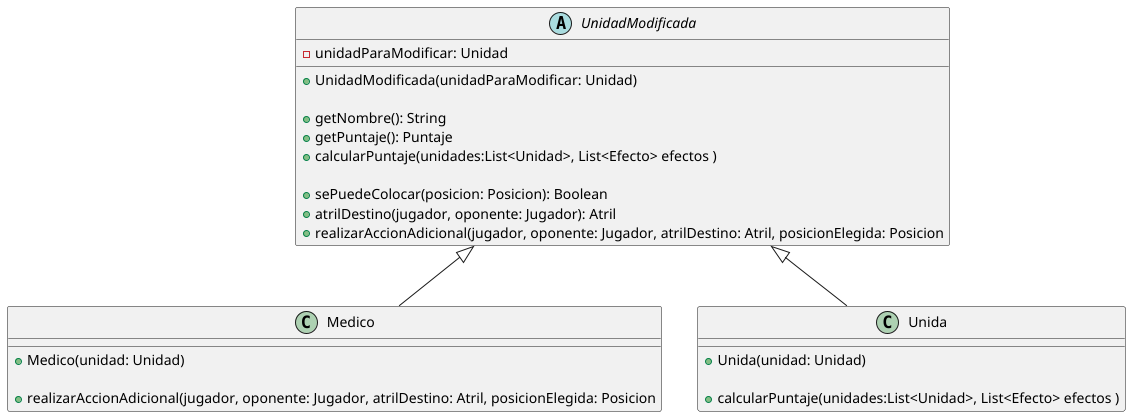
\includegraphics[width=1\textwidth]{diagramas/clases/Modificadores3}
		\caption{\label{fig:class083}Cartas unidad \texttt{Modificadores}.}
	\end{figure}

	\begin{figure}[H]
		\centering
		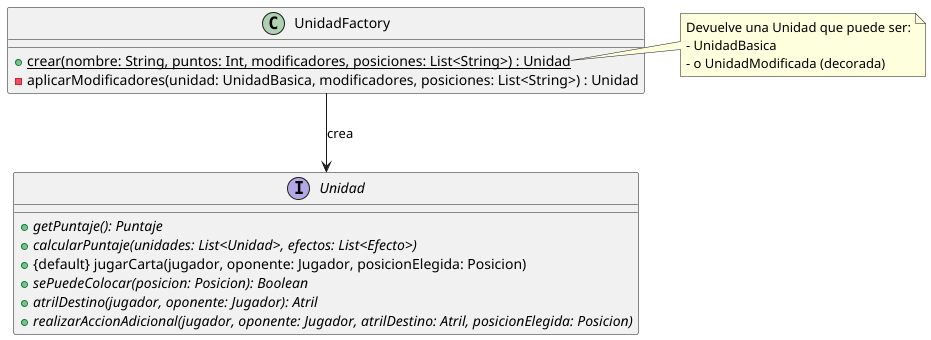
\includegraphics[width=1\textwidth]{diagramas/clases/UnidadFactory}
		\caption{\label{fig:class09} \texttt{UnidadFactory}.}
	\end{figure}

	\subsection{Diagramas de secuencia}\label{sec:diagramasdesecuencia}
	% Mostrar las secuencias interesantes que hayan implementado. Pueden agregar texto para explicar si algo no queda claro.

	\subsection{Secuencia: Jugar carta de unidad con modificador Espía}
	Vamos a mostrar una secuencia de como se juega una \textbf{carta de unidad con el modificador \textit{Espia}} en la posicion \textbf{Asedio}.

	\begin{figure}[H]
		\centering
		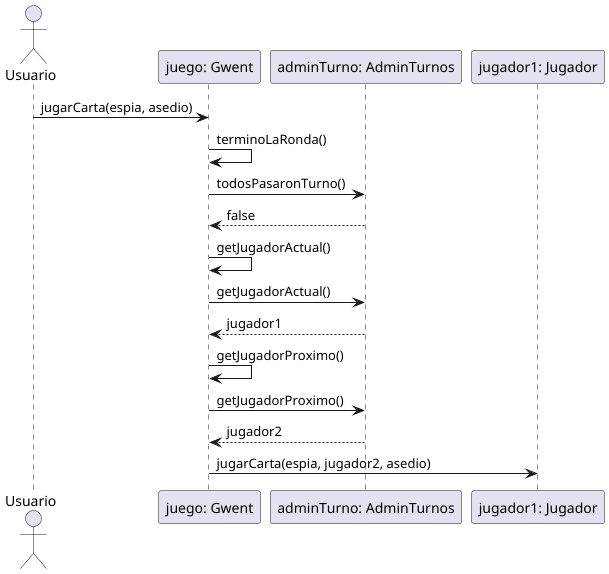
\includegraphics[width=1\textwidth]{diagramas/secuencia/jugarCarta1}
		\caption{\label{fig:secuencia01} validación de la ronda y turno del jugador.}
	\end{figure}
	A nivel del juego de Gwent, antes de jugar una carta se valida que \textbf{la ronda no haya terminado}, y se determina \textbf{quién debe jugar} la carta, dependiendo de a quién le corresponde el turno actual.

	\begin{figure}[H]
		\centering
		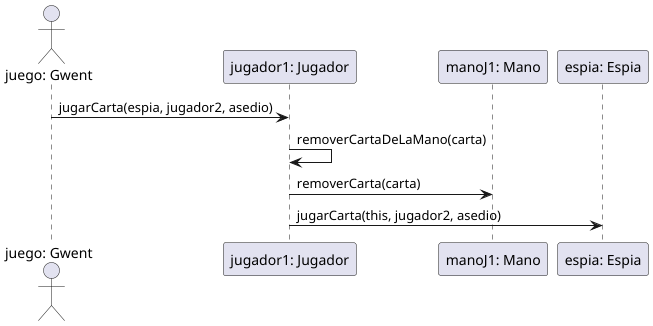
\includegraphics[width=1\textwidth]{diagramas/secuencia/JugarCarta2}
		\caption{\label{fig:secuencia02} Jugador juega carta}
	\end{figure}
	En esta etapa, el \texttt{Jugador} valida que la carta que se intenta jugar \textbf{pertenezca a su mano}. El método \texttt{removerCartaDeLaMano()} puede lanzar una excepción en caso de que la carta no esté disponible en la mano del jugador.

	\begin{figure}[H]
		\centering
		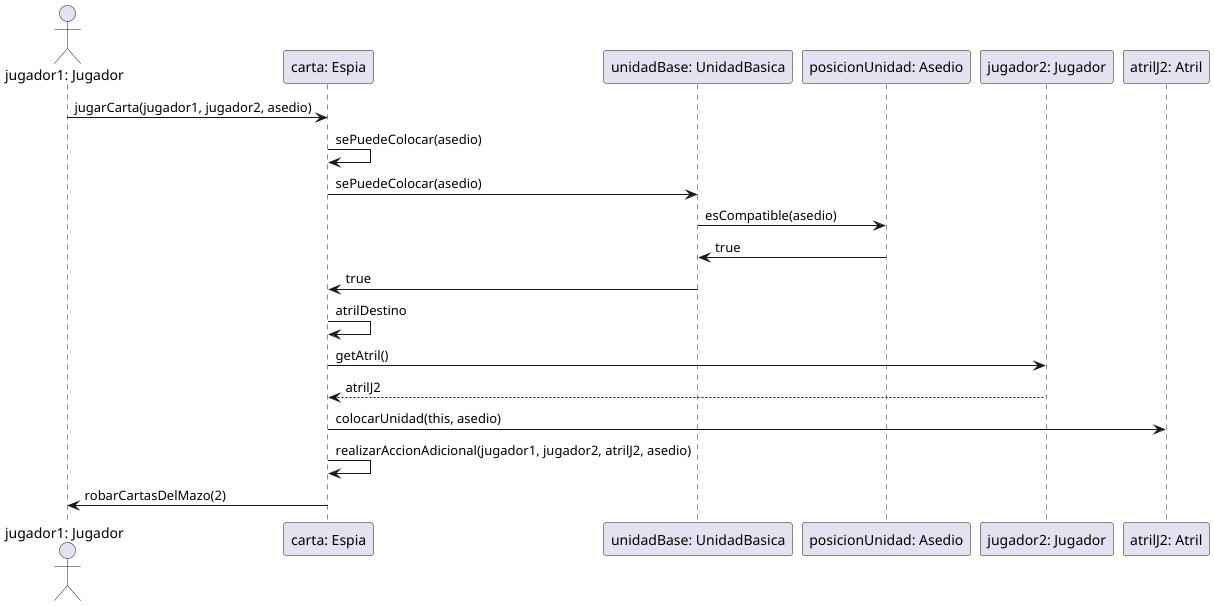
\includegraphics[width=1\textwidth]{diagramas/secuencia/jugarCarta3}
		\caption{\label{fig:secuencia03} modificador \textit{Espia}}
	\end{figure}
	En esta parte de la secuencia se muestra cómo el \textbf{modificador \textit{Espía}} altera el comportamiento de la carta: \textbf{cambia el atril de destino} (haciéndola jugar en el lado del oponente) y provoca que el jugador que la juega \textbf{robe 2 cartas} de su propio mazo luego de que la carta es colocada.

	\begin{figure}[H]
		\centering
		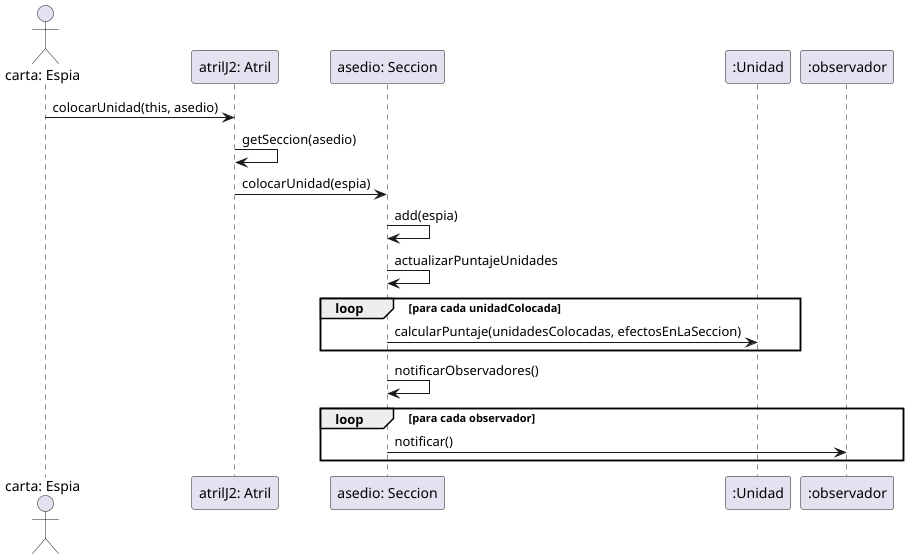
\includegraphics[width=1\textwidth]{diagramas/secuencia/jugarCarta4}
		\caption{\label{fig:secuencia04} Actualizacion del puntaje y notificacion a los observadores}
	\end{figure}
	Finalmente, al colocar una unidad en una sección, se actualiza el puntaje actual de las \textbf{unidades colocadas}. Además, se notifica a los \textbf{observadores} registrados en la sección.



\end{document}